\begingroup
\examsetup{February 13, 2018}{Spring 2018}
\vspace*{1.0in}
\begin{center}
{\sffamily\bfseries\fontsize{16}{20}\selectfont
Texas A\&M University\\
Department of Electrical and Computer Engineering\par}
\vspace{.40in}
{\sffamily\bfseries\fontsize{15}{18}\selectfont
ECEN 474/704 -- (Analog) VLSI Circuit Design\par}
\vspace{.38in}
{\sffamily\bfseries\fontsize{16}{19}\selectfont Spring 2018\par}
\vspace{.30in}
{\sffamily\bfseries\fontsize{16}{19}\selectfont Exam \#1\par}
\vspace{.30in}
{\sffamily\bfseries\fontsize{16}{19}\selectfont Instructor: Sam Palermo\par}
\end{center}
\vspace{.42in}
\begin{itemize}[leftmargin=.3in,itemsep=1pt,topsep=0pt]
\item Please write your name in the space provided below
\item Please verify that there are \textbf{6 pages} in your exam
\item You may use \underline{one} double-sided page of notes and equations for the exam
\item Good Luck!
\end{itemize}
\vspace{.65in}
\begin{tabular}{|c|c|c|}\hline
Problem&Score&Max Score\\\hline
1&&40\\\hline
2&&40\\\hline
3&&20\\\hline
\textbf{Total}&&\textbf{100}\\\hline
\end{tabular}
\vfill
Name: \hrulefill\par
\vspace{7pt}
UIN: \hrulefill
\vspace{.12in}

\newpage
{\fontsize{10.7}{12.2}\selectfont
\textbf{Problem 1 (40 points)}\par
For the layout below, assume that all the commonly labeled diffusion areas
are connected with the appropriate metal layers. Assume that
$V_A=2\,\mathrm V$, $V_B=1.5\,\mathrm V$, $V_C=1.0\,\mathrm V$,
$V_{T0}=0.7\,\mathrm V$, $\gamma=0$, and that all Spice parameters are given
(i.e.\ $C_j,C_{jsw},C_{jc},C_{ox},C_{ov}$). The dimensions are given in
$\mu\mathrm m$, with the poly gates having $L_D=0.1\,\mu\mathrm m$.
\begin{enumerate}[label=\alph*),leftmargin=.25in,itemsep=1pt,topsep=2pt]
\item Draw the equivalent circuit. Combine all parallel transistors and give
the total width and length of the equivalent transistors.
\item What region(s) are the transistors operating in?
\item \textbf{For node B only,} give an expression and calculate the total
gate cap (only consider where B is the gate).
\item \textbf{For node A only,} give an expression and calculate the total
junction cap, including the relevant channel-bulk cap.
Note for the perimeter terms, include the sides underneath the gate.
\end{enumerate}
\begin{center}
\begin{tikzpicture}[x=.78cm,y=.78cm,font=\scriptsize]
\draw (-.6,-.75) rectangle (10.7,3.7);
\node[anchor=west]at(-.3,3.35){P-sub};
\fill[black!80](1.3,3.25)rectangle(1.55,3.5);
\node[anchor=west]at(1.65,3.37){Poly};
\fill[black](3.25,3.25)rectangle(3.48,3.48);
\node[anchor=west]at(3.6,3.37){Contact (poly or diffusion)};
\draw[pattern=grid,pattern color=black!60](1.3,2.75)rectangle(1.55,3);
\node[anchor=west]at(1.65,2.87){N+};
\fill[black!15](3.25,2.75)rectangle(3.5,3);
\node[anchor=west]at(3.6,2.87){M1};
\draw[pattern=grid,pattern color=black!45](-.05,.05)rectangle(9.85,1.5);
\foreach \i/\lab in {0/C,1/A,2/C,3/B,4/C,5/B,6/C,7/A,8/C}{
 \pgfmathsetmacro{\xx}{.3+1.15*\i}
 \fill[white](\xx-.09,.25)rectangle(\xx+.38,1.3);
 \fill(\xx,.27)rectangle(\xx+.22,.49);
 \fill(\xx,1.05)rectangle(\xx+.22,1.27);
 \node[font=\bfseries\scriptsize]at(\xx+.11,.78){\lab};
}
\foreach \i in {0,1,6,7}{
 \pgfmathsetmacro{\xx}{.86+1.15*\i}
 \fill[black!80](\xx,.02)rectangle(\xx+.20,1.78);
}
\foreach \i in {2,3,4,5}{
 \pgfmathsetmacro{\xx}{.86+1.15*\i}
 \fill[black!80](\xx,-.23)rectangle(\xx+.20,1.65);
}
\fill[black!80](.86,1.78)rectangle(9.11,2.0);
\fill[black!80](.86,-.23)rectangle(9.11,-.01);
\foreach \i in {3,5}{
 \pgfmathsetmacro{\xx}{.3+1.15*\i}
 \fill[black!15](\xx-.05,1.05)rectangle(\xx+.27,2.10);
 \fill(\xx,1.05)rectangle(\xx+.22,1.27);
 \fill(\xx,1.78)rectangle(\xx+.22,2.0);
}
\foreach \i in {1,7}{
 \pgfmathsetmacro{\xx}{.3+1.15*\i}
 \fill[black!15](\xx-.05,-.35)rectangle(\xx+.27,.49);
 \fill(\xx,.27)rectangle(\xx+.22,.49);
 \fill(\xx,-.23)rectangle(\xx+.22,-.01);
}
\draw[<->](-.3,.05)--node[left]{10}(-.3,1.5);
\draw[<->](.02,-.48)--node[below]{6}(.77,-.48);
\draw[<->](.87,-.48)--node[below]{2}(1.07,-.48);
\draw[<->](1.07,2.17)--node[above]{6}(1.82,2.17);
\node[anchor=west]at(5.3,2.43){Diffusion spacing: 6};
\end{tikzpicture}
\end{center}
\vspace{-6pt}
\textbf{Typeset solution.}
All eight individual transistors have $W/L=10/2$.
Four parallel devices form each equivalent transistor:
\begin{center}
\begin{circuitikz}[scale=.8,transform shape]
\node[nmos] (m1) at (1.3,0) {};
\node[nmos,xscale=-1] (m2) at (5,0) {};
\draw (m1.S)--(1.3,-1.2)--(5,-1.2)--(m2.S);
\node[below] at (3.1,-1.2){$C=1.0\,\mathrm V$};
\draw (m1.D)--(1.3,1.0) node[above]{$A=2.0\,\mathrm V$};
\draw (m2.D)--(5,1.0) node[above]{$B=1.5\,\mathrm V$};
\draw (m1.G)--(-.4,0) node[left]{$B$};
\draw (m2.G)--(6.7,0) node[right]{$A$};
\node[below]at(1.3,-1.65){$M_1:\ W/L=40/2$};
\node[below]at(5,-1.65){$M_2:\ W/L=40/2$};
\end{circuitikz}
\end{center}
\vspace{-8pt}
\begin{align*}
M_1:\quad &V_{GS}=1.5-1.0=0.5\,\mathrm V<V_T
&&\Longrightarrow\ \boxed{\text{cutoff or subthreshold}},\\
M_2:\quad &V_{GS}=2.0-1.0=1.0\,\mathrm V>V_T,\quad
V_{DS}=0.5\,\mathrm V>V_{GS}-V_T=0.3\,\mathrm V
&&\Longrightarrow\ \boxed{\text{saturation}}.
\end{align*}
For B, $M_1$ is cut off. With $L_{\rm eff}=2-2(0.1)=1.8\,\mu\mathrm m$,
\[
C_{gB}=C_{gc}+C_{gs,ov}+C_{gd,ov}
=(40\,\mu\mathrm m)(1.8\,\mu\mathrm m)
\frac{C_{ox}C_{jc}}{C_{ox}+C_{jc}}+2(40\,\mu\mathrm m)C_{ov},
\]
\[
\boxed{C_{gB}=72\,\mu\mathrm m^2\frac{C_{ox}C_{jc}}{C_{ox}+C_{jc}}
+80\,\mu\mathrm m\,C_{ov}.}
\]
For A, the two $10\times6$ diffusion regions give
\[
C_{jA}=A_A C_j+P_A C_{jsw}
=2(10)(6)\,\mu\mathrm m^2C_j+2\,[2(10+6)]\,\mu\mathrm m\,C_{jsw},
\qquad
\boxed{C_{jA}=120\,\mu\mathrm m^2C_j+64\,\mu\mathrm m\,C_{jsw}.}
\]
}

\newpage
{\fontsize{10.7}{12.2}\selectfont
\textbf{Problem 2 (40 points)}\par
For the circuit shown below, assume the transistor has
$V_{T0}=0.7\,\mathrm V$, $\gamma=0.45\,\mathrm V^{1/2}$, and
$2\Phi_F=0.9\,\mathrm V$, and its DC drain current is determined by the following equations.
\begin{center}
\begin{minipage}{.36\linewidth}\centering
\begin{circuitikz}[scale=.82,transform shape]
\node[nmos,bulk] (m) at (1.5,2) {};
\draw (m.D)--(1.5,3.3) node[above]{$1.0\,\mathrm V$};
\draw (.95,2.6)node[left]{$\dfrac{10\,\mu\mathrm m}{1\,\mu\mathrm m}$};
\draw (m.G)--(-.35,2) to[sV,l_=$v_i$](-.35,.8)
 to[V,l_=$1.9\,\mathrm V$](-.35,-.7) node[ground]{};
\draw (m.S)--(1.5,.9) node[circ]{};
\node[anchor=west]at(1.7,1.25){$V_{S,Q}=0.8\,\mathrm V$};
\draw (1.5,.9)to[I,l_=$I_B$](1.5,-.7)node[ground]{};
\draw (1.5,.9)to[C](3.3,.9)node[circ]{}--(3.7,.9)node[right]{$v_o$};
\draw (3.3,.9)to[R,l=$R_L$](3.3,-.7)node[ground]{};
\draw (m.bulk)--++(.35,0)node[ground]{};
\end{circuitikz}
\end{minipage}\hfill
\begin{minipage}{.61\linewidth}\fontsize{9.4}{11.5}\selectfont
\begin{align*}
I_{DS}&=I_o\exp\!\left(\frac{(V_{GS}-V_{Tn})q}{\zeta kT}\right)
\left[1-\exp\!\left(-\frac{V_{DS}q}{kT}\right)\right]
&&\text{(Subthreshold)},\\[4pt]
I_{DS}&=\mu_n C_{ox}\frac{W}{L-2L_D}
\left(V_{GS}-V_{Tn}-0.5V_{DS}\right)V_{DS}
&&\text{(Triode)},\\[4pt]
I_{DS}&=\frac12\mu_n C_{ox}\frac{W}{L-2L_D}
\left(V_{GS}-V_{Tn}\right)^2(1+\lambda V_{DS})
&&\text{(Saturation)},\\[4pt]
V_{Tn}&=V_{T0}+\gamma\left(\sqrt{|2\Phi_F|+V_{SB}}-\sqrt{|2\Phi_F|}\right).
\end{align*}
\end{minipage}
\end{center}
\textbf{a.}\quad Calculate $V_T$ and state the transistor's operation region.
\begin{align*}
V_T&=0.7+0.45\left(\sqrt{0.9+0.8}-\sqrt{0.9}\right)
=\boxed{0.860\,\mathrm V},\\
V_{DS}&=0.2\,\mathrm V,\qquad
V_{GS}-V_T=1.1-0.86=0.24\,\mathrm V,\\
V_{DS}&<V_{GS}-V_T\quad\Longrightarrow\quad
\boxed{\text{Operation region: Triode}.}
\end{align*}
\textbf{b.}\quad Using the appropriate $I_{DS}$ equation above,
\textbf{draw the low-frequency small-signal model of the circuit}
(neglecting transistor capacitors), \textbf{include expressions for
$g_m$, $g_o$ and $g_{mb}$, and give an expression for the small-signal
voltage gain} $A_v=v_o/v_i$ in terms of the relevant transistor
conductances and load resistor. Assume the output AC-coupling capacitor
acts as an ideal short.

\begin{minipage}[t]{.49\linewidth}
\begin{align*}
g_m&=\left.\frac{\partial I_{DS}}{\partial V_{GS}}\right|_Q
=\mu_n C_{ox}\frac{W}{L_{\rm eff}}V_{DS},\\[4pt]
g_o&=\left.\frac{\partial I_{DS}}{\partial V_{DS}}\right|_Q\\
&=\mu_n C_{ox}\frac{W}{L_{\rm eff}}
(V_{GS}-V_T-V_{DS}),\\[4pt]
g_{mb}&=\left.\frac{\partial I_{DS}}{\partial V_{BS}}\right|_Q\\
&=\mu_n C_{ox}\frac{W}{L_{\rm eff}}V_{DS}
\frac{\gamma}{2\sqrt{|2\Phi_F|+V_{SB}}}\\
&=\frac{\gamma g_m}{2\sqrt{|2\Phi_F|+V_{SB}}}=\eta g_m.
\end{align*}
\end{minipage}\hfill
\begin{minipage}[t]{.47\linewidth}
\vspace{10pt}\centering
\begin{circuitikz}[scale=.82,transform shape]
\draw (0,0)node[ground]{}--(5.4,0);
\draw (0,0)to[cI,l_={$g_m(v_i-v_o)$}](0,-1.9);
\draw (2.7,0)to[cI](2.7,-1.9);
\node[above]at(2.7,.15){$g_{mb}(-v_o)$};
\draw (5.4,0)to[R,l=$r_o$](5.4,-1.9);
\draw (0,-1.9)--(5.4,-1.9);
\draw (2.7,-1.9)node[circ]{}node[right]{$v_o$}
 to[R,l=$R_L$](2.7,-3.2)node[ground]{};
\end{circuitikz}
\end{minipage}
\begin{align*}
v_o&=\left[g_m(v_i-v_o)+g_{mb}(-v_o)\right](R_L\parallel r_o),\\
v_o\left[1+(g_m+g_{mb})(R_L\parallel r_o)\right]
&=v_i g_m(R_L\parallel r_o),\\
\boxed{\frac{v_o}{v_i}}
&\boxed{=\frac{g_m(R_L\parallel r_o)}{1+(g_m+g_{mb})(R_L\parallel r_o)}.}
\end{align*}
}

\newpage
\textbf{c.}\quad In addition to the parameters given previously, assume
$I_o=1\,\mathrm{nA}$, $kT/q=25.9\,\mathrm{mV}$, $\zeta=1$,
$\mu_n C_{ox}=130\,\mu\mathrm A/\mathrm V^2$,
$L_D=0.1\,\mu\mathrm m$, and $\lambda=0.1\,\mathrm V^{-1}$.
Calculate the necessary load resistor for $|A_v|=0.7\,\mathrm{V/V}$.
\vspace{.30in}
\begin{align*}
A_v&=\frac{g_m(R_L\parallel r_o)}{1+(g_m+g_{mb})(R_L\parallel r_o)}
=\frac{g_m}{G_L+g_o+(1+\eta)g_m},\\[14pt]
G_L&=\frac{g_m}{A_v}-g_o-(1+\eta)g_m,\\[20pt]
g_m&=(130\,\mu)\left(\frac{10}{0.8}\right)(0.2)
=325\,\mu\mathrm A/\mathrm V,\\[18pt]
g_o&=(130\,\mu)\left(\frac{10}{0.8}\right)(1.1-0.86-0.2)
=65\,\mu\mathrm A/\mathrm V,\\[18pt]
\eta&=\frac{0.45}{2\sqrt{0.9+0.8}}\simeq0.173,\\[20pt]
G_L&=\frac{325\,\mu}{0.7}-65\,\mu-1.173(325\,\mu)
\simeq18.1\,\mu\mathrm A/\mathrm V,\\[20pt]
R_L&=\frac{1}{G_L}\simeq\boxed{55.4\,\mathrm{k}\Omega}.
\end{align*}
\vspace{.35in}
{\small\textit{Rounding note:} the supplied solution rounds $V_T$, $g_o$,
and $\eta$ before computing $G_L$. Retaining their full values gives
$R_L\simeq55.83\,\mathrm{k}\Omega$; the displayed $55.4\,\mathrm{k}\Omega$
reproduces the supplied rounded calculation.}
\vfill
\hfill $R_L\text{ for }|A_v|=0.7\,\mathrm{V/V}=55.4\,\mathrm{k}\Omega$
\vspace{.12in}

\newpage
{\fontsize{10.7}{12.3}\selectfont
\setlength{\parskip}{3pt}
\setlength{\abovedisplayskip}{4pt}
\setlength{\belowdisplayskip}{4pt}
\setlength{\jot}{2pt}
\textbf{Problem 3 (20 points)}\par
The layout of a simple RC-filter is shown below. For the 3-finger resistor,
assume $R_{\square}=200\,\Omega/\square$ and each contact has a resistance
of $10\,\Omega$. The capacitor consists of 4 unit capacitors that each have
top-plate dimensions of $10\,\mu\mathrm m\times10\,\mu\mathrm m$.
These unit capacitors have a capacitive density of $1\,\mathrm{fF}/\mu\mathrm m^2$.
\begin{enumerate}[label=\alph*.,leftmargin=.25in,itemsep=1pt,topsep=2pt]
\item Sketch the equivalent circuit and give the values of the resistor and
capacitor. The resistor contacts should be included in its resistance
calculation, but the capacitor contacts' resistance may be ignored.
Neglect the impedance of all metal interconnect between the elements.
\item Sketch the Bode plot (magnitude only), and label any pole and/or zero frequencies.
\end{enumerate}
\begin{minipage}[t]{.45\linewidth}\vspace{0pt}\centering
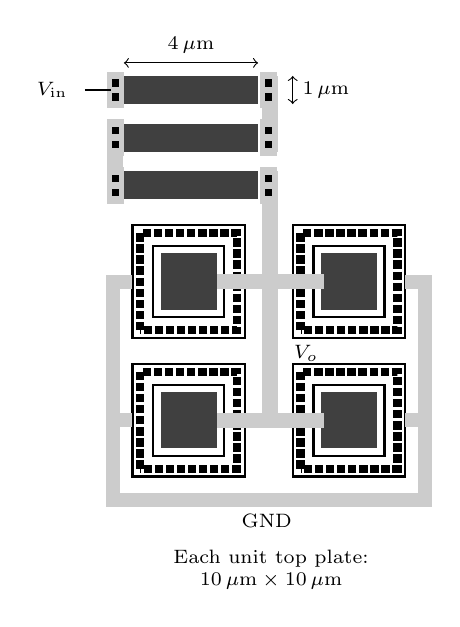
\begin{tikzpicture}[x=.55cm,y=.55cm,font=\scriptsize]
\foreach \yy in {6.5,5.4,4.3}{
 \fill[black!75](.8,\yy)rectangle(3.9,\yy+.65);
 \foreach \xx in {.52,4.05}{
   \fill[black!20](\xx-.10,\yy-.1)rectangle(\xx+.28,\yy+.75);
   \fill(\xx,\yy+.08)rectangle(\xx+.17,\yy+.25);
   \fill(\xx,\yy+.40)rectangle(\xx+.17,\yy+.57);
 }
}
\fill[black!20](4.0,5.4)rectangle(4.35,7.15);
\fill[black!20](.42,4.3)rectangle(.77,6.05);
\fill[black!20](4.0,2.5)rectangle(4.35,4.95);
\draw[<->](.8,7.45)--node[above]{$4\,\mu\mathrm m$}(3.9,7.45);
\draw[<->](4.7,6.5)--node[right]{$1\,\mu\mathrm m$}(4.7,7.15);
\draw[thick](-.1,6.83)--(.5,6.83) node[left,xshift=-12pt]{$V_{\rm in}$};
\foreach \xx in {1.0,4.7}{\foreach \yy in {1.1,-2.1}{
 \draw[thick](\xx,\yy)rectangle(\xx+2.6,\yy+2.6);
 \draw[densely dotted,line width=3pt](\xx+.18,\yy+.18)rectangle(\xx+2.42,\yy+2.42);
 \draw[thick](\xx+.48,\yy+.48)rectangle(\xx+2.12,\yy+2.12);
 \fill[black!75](\xx+.65,\yy+.65)rectangle(\xx+1.95,\yy+1.95);
}}
\fill[black!20](2.95,2.23)rectangle(5.42,2.57);
\fill[black!20](2.95,-.97)rectangle(5.42,-.63);
\fill[black!20](4.0,-.97)rectangle(4.35,4.95);
\node[anchor=west]at(4.5,.75){$V_o$};
\draw[line width=5pt,black!20](1,2.4)--(.55,2.4)--(.55,-2.65)
 --(7.75,-2.65)--(7.75,2.4)--(7.3,2.4);
\draw[line width=5pt,black!20](1,-.8)--(.55,-.8);
\draw[line width=5pt,black!20](7.3,-.8)--(7.75,-.8);
\foreach \yy in {6.5,5.4,4.3}{\foreach \xx in {.52,4.05}{
 \fill(\xx,\yy+.08)rectangle(\xx+.17,\yy+.25);
 \fill(\xx,\yy+.40)rectangle(\xx+.17,\yy+.57);
}}
\node[below]at(4.1,-2.75){GND};
\node[align=center]at(4.2,-4.25){Each unit top plate:\\$10\,\mu\mathrm m\times10\,\mu\mathrm m$};
\end{tikzpicture}
\end{minipage}\hfill
\begin{minipage}[t]{.52\linewidth}\vspace{0pt}
\textbf{Typeset solution.}\par
$n$ is the number of parallel contacts at each end;
$F$ is the number of resistor fingers.
\begin{align*}
R_{\rm total}&=\left(\frac{2R_c}{n}+R_{\square}\frac{L}{W}\right)F\\[2pt]
&=\left[\frac{2(10)}2+200\left(\frac41\right)\right]3\\[2pt]
&=\boxed{2.43\,\mathrm{k}\Omega}.
\end{align*}
With $U=4$ unit capacitors,
\begin{align*}
C_{\rm total}&=A_{\rm top}C_{\rm density}U\\
&=(10\,\mu\mathrm m)(10\,\mu\mathrm m)
\left(1\,\frac{\mathrm{fF}}{\mu\mathrm m^2}\right)4\\
&=\boxed{400\,\mathrm{fF}}.
\end{align*}
\begin{center}
\begin{circuitikz}[scale=.72,transform shape]
\draw (0,0)node[left]{$V_{\rm in}$}to[R,l=$2.43\,\mathrm{k}\Omega$](3,0)
 node[circ]{}--(4,0)node[right]{$V_o$};
\draw (3,0)to[C,l=$400\,\mathrm{fF}$](3,-1.6)node[ground]{};
\end{circuitikz}
\end{center}
\begin{align*}
\frac{V_o}{V_i}&=\frac{1}{1+sRC}
=\frac{1}{1+s(9.72\times10^{-10}\,\mathrm s)},\\
A_{\rm DC}&=1=0\,\mathrm{dB},\\
\omega_p&=-\frac1{RC}\simeq-1.03\times10^9\,\mathrm{rad/s},\\
f_p&=\frac1{2\pi RC}\simeq\boxed{164\,\mathrm{MHz}}.
\end{align*}
\end{minipage}
\vspace{4pt}
\begin{center}
\begin{tikzpicture}[x=1cm,y=.85cm,font=\small]
\draw[-{Latex}](0,0)--(9,0)node[right]{$f$ (Hz, logarithmic)};
\draw[-{Latex}](0,-.15)--(0,2.35)node[above]{Magnitude (dB)};
\draw[thick](0,1.8)--(3,1.8)--(8,.25);
\draw[dashed](3,0)--(3,2);
\node[left]at(0,1.8){0};
\node[below]at(3,0){$164\,\mathrm{MHz}$};
\node[above,rotate=-17]at(6,1.12){$-20\,\mathrm{dB/decade}$};
\node[below]at(7.1,-.55){One pole; no finite zero};
\end{tikzpicture}
\end{center}
}

\newpage
\begin{center}
{\sffamily\bfseries\fontsize{16}{20}\selectfont Scratch Paper}
\end{center}
\vfill\mbox{}
\clearpage
\endgroup
